\section{Constructing a National Certification Program}

\emph{Julie Cease}

\subsection{Introduction}
The Federal Government currently either owns or leases over 3 billion square feet of building space. A small but expanding number of alternative energy-focused federal facilities has already demonstrated proof of concept in minimizing the federal facility energy consumption footprint. Within the US General Services Administration (GSA), the Office of Federal High-Performance Green Buildings has been authorized by Congress under the Energy Independence and Security Act (EISA) to promote and to expand Federal participation in sustainable property development. Since its inception, the Office of Federal High-Performance Green Buildings has overseen more than 2,500 projects, all certified through the US Green Building Council’s Leadership in Energy and Environmental Design (LEED) program. The purpose of this report is to outline a detailed implementation plan whose objectives are to document a Federal Rooftop Solar Certification Program with strategic emphasis on (1) providing a roadmap for a certification system of national import, and (2) incorporating material criticality concerns where appropriate within the principles of best practice.


\subsection{Developing a Federal Rooftop Solar Certification Program}
Currently, LEED represents the principle system for rating sustainable design measures under the US Green Building Council directive. The Green Building Certification System Review published in March 2012 and prepared by the US Department of Energy (DOE) in accordance with EISA § 433(a) and 426(h) specifies EISA-sanctioned criteria to be used in reviewing certification systems. Specifically, the certification systems must meet three standards both for new construction and for existing buildings; (1) they must employ whole building evaluation, addressing key sustainable design and operations metrics, (2) they must be available in the US market, and (3) they must have third party certification. Whereas the afore mentioned methodology presents screening criteria for green building designs as a whole, the solar photovoltaic mandate proposed here, because it regards rooftop installation alone, will address the last two criteria for determining the minimum system requirements for Federal Building solar photovoltaic installations. The recommendations to follow fall under the EISA rubric and adhere to the EISA criteria.


\subsubsection{Technologies and Feasibility Study}
The first phase of certification will entail a technologies and feasibility study to be conducted by a third-party auditor responsible for performing onsite rooftop and general location-centered evaluation. The Green Building Certification Institute (GBCI) will provide third-party certification. Site and structural assessment as well as all documentation to be submitted in response to site evaluation and verification will be undertaken within the official auspices of the GBCI. For this review, the following considerations will be assessed:

\begin{itemize}
\item Extant Neighborhood
\item Landscape Infrastructure
\item Insolation Potential
\end{itemize}

The purpose of the Technologies and Feasibility Study is to screen proposed and existing properties for both for future optimization and for resultant impracticable obstacles that may interfere with the installation of a solar energy system. The scope of such a study includes an evaluation of the extant neighborhood, which includes the urban block(s) surrounding the proposed site, along with the general landscape geometry, which enables mapping of discrete sky verses shadow segments impinging on future installation infrastructure. The urban block(s) surrounding a proposed site may impose significant influence on solar access. Tall residential and commercial buildings produce shading masks throughout a solar day. Geometric topography of neighboring buildings combined with varied solar heights at local latitudes across the United States will of necessity converge to produce diverse access conditions, all of which will dictate the feasibility of a particular solar photovoltaic installation.
\\\\
\noindent Sustainable building design software offers detailed and highly analytical profiling of either existing or proposed sites from the earliest stages of architectural design. Autodesk Ecotect Analysis is one program that enables multiplexing of disparate data streams into a composite energy picture. Figure \ref{juliefig1} shows an Ecotect analysis example, in which data sets including building typology, lighting simulation, solar insolation, direct shading, and seasonal climate analysis can be combined in an interpolated 3D visualization of the target site.

\begin{figure}
\begin{center}
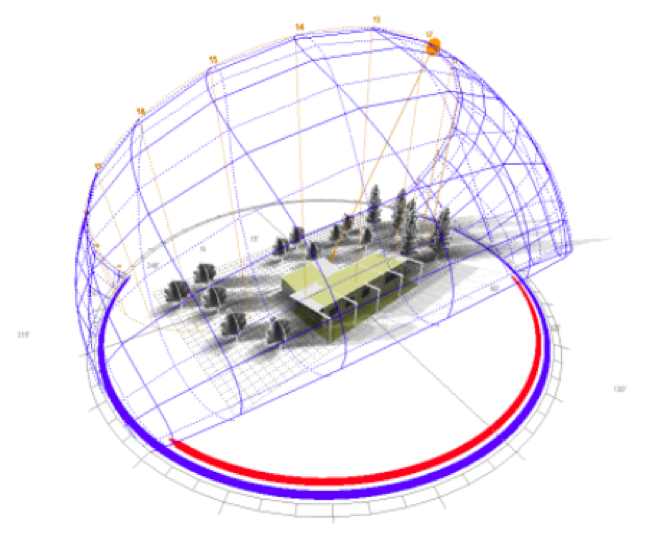
\includegraphics[scale=0.7]{julie_pic_1.png}
\caption{Ecotect analysis example}
\label{juliefig1}
\end{center}
\end{figure}


\subsubsection{Alternatives Evaluation}
The second phase of certification involves an evaluation of alternatives. As with the Technologies and Feasibility Study presented above in Phase One, the Green Building Certification Institute (GBCI) will provide third-party assessment of alternatives. Alternative considerations will include:

\begin{itemize}
\item Financing Options
\item Weathering
\item Module Specification
\end{itemize}

Consistent with a mandate seeking to provide maximum flexibility and adaptability where site-specific implementation is concerned, three financing options come under consideration: cash purchase, power purchase agreement (PPA), and lease. A cash purchase option entails a one-time upfront purchase cost where the purchaser owns the system hardware. Progress payments occur coincident with construction progress. The option to lease a rooftop solar photovoltaic system demands zero or low upfront cost, but requires a recurring lease payment combined with a fixed payment for the system hardware. The PPA represents a versatile option wherein the purchaser incurs no upfront cost but pays a fixed rate for energy in the form of payment per kWh consumed.
\\\\
\noindent Due to incomparable climactic variation across the US, issues of module weatherability arise. Module producers typically guarantee photovoltaic panels for 20 to 25 years, with warranty coverage specifying performance of at least 90\% capacity for the first ten years and at least 80\% capacity for the remaining fifteen years. All photovoltaic module designs must undergo testing in accordance with the International Electrotechnical Commission (IEC) for qualification of design, materials, and defects. Wafer based silicon is certified under IEC 61215 whereas thin film technologies undergo qualification under IEC 61646. Importantly, neither of these qualification regimes subject models to test protocols that include or combine weather exposure testing—even though both formal laboratory and outdoor accelerated weather testing is available.


\paragraph{Evaluating Extreme Service Environments} \mbox{ }\\
Within the continental US, Alaska and Hawaii, three extreme service environments exist: desert/monsoonal, tropical, and polar. Taking data from the Technologies and Feasibility study described above for Phase One, modules targeted for deployment in extreme service environment climatic regions must undergo advanced durability testing prior to certification. Unlike IEC testing, which focuses on design type qualification tests, which are engineered to identify short-term failure, Accelerated Environmental Testing (AET) reproduces likely field conditions using a set of comprehensive climate stresses. Stress testing comprised of multiple simultaneous loads including temperature, humidity, salt spray, extreme UV, freeze-thaw cycling, and maximum power draw produces accumulated damage and field failure representative of long-term outdoor extreme exposure. The weathering testing proposed here is based on a global composite climate standard compiled under the Köppen-Geiger climate classification system. This climate map is used to predict geographic regions situated within worst-case climate boundary conditions.
\\\\
\noindent Alternatives decisions with respect to module selection and orientation can accommodate a wide array of rooftop configurations and site-specific insolation patterns. Solar panel selection, however, will need to come from top tier producers if robustness and efficiency are to be maintained throughout the mandate. Modules produced in the US must comply with competitive best practice dynamics in terms of research and development, material quality, production processing and energy conversion efficiency. Pike Research, a market research firm based in Boulder, Colorado, specializing in providing rigorous technical analysis of global clean technology trends, recently published a tier system whereby global solar photovoltaic module producers achieve a general rank according to in-house versus outsourcing of manufacturing processes, investment in research and development, manufacturer longevity, and stringent quality control. Price to consumer plays no role in the ranking system.

\paragraph{Tier One Module Producers}\mbox{ }\\
Tier 1 solar photovoltaic modules represent panels fabricated from the top 5\% of solar manufacturers. Tier 1 producers control all stages of module manufacture in a vertically integrated production process. Photovoltaic modules, whether based on silicon or thin film technologies, begin component level deposition or build-up in-house and remain in- house through the entire production process—through panel assembly and module framing to installation and warranty. Tier 1 ranked producers invest consistently and comprehensively in research and development. Hence, these module manufacturers often lead the industry in offering state-of-the-art innovation in both process and product. Furthermore, Tier 1 manufacturers employ advanced robotic fabrication techniques with demonstrated correlation to engineering quality. Robotic fabrication not only reflects a low margin of off-specification product due to device defect and failure, it reduces critical material in the industrial waste stream. Lastly, Tier 1 producers must demonstrate longevity in a relatively young industry through viable commercial manufacture of solar photovoltaics for a minimum of 5 years.

\paragraph{Tier Two Module Producers}\mbox{ }\\
Whereas Tier 1 modules typically lead the industry with electrical conversion efficiencies above 21\%, Tier 2 modules operate at competitive efficiencies of 15\% or greater. Tier 2 panels are considered to be within roughly the top 20\% of all modules produced, although the manufacturers represent approximately 8\% of the solar photovoltaic production market share. Producers ranked within Tier 2 typically account for the best small to medium scale manufacturers. These are the producers who fabricate good quality modules, but whose assembly and production processes take place only partially in-house. Tier 2 producers rely primarily on manual labor in addition to robotic assembly and test of cells in production. Even though the grade and type of silicon or the elements in a thin film cells may be identical to those deployed in the manufacture of Tier 1 cells, off-spec modules and semiconductor grade scrap materials will enter the industrial waster stream at a higher rate for Tier 2 fabrication and production lines. Unlike Tier 1 producers, who drive innovation, Tier 2 producers generally invest little in research and development, having typically between 2 to 5 years production experience in photovoltaic manufacture.

\paragraph{Tier Three and Other Module Producers}\mbox{ }\\
Whereas Tier 3 companies comprise the bulk of the manufacturing market, these solar photovoltaic manufacturers employ only limited robotics and no advanced production technologies in their manufacturing operations. By and large, Tier 3 producers simply assemble solar panels. Since these companies neither produce silicon cells nor fabricate thin films in-house but rely nearly exclusively on manual labor to construct modules, quality and durability in their product lines can vary widely. Not only do solar cell components that have been produced by hand lack the consistent and reliable quality control of an automated system, the devices themselves lack the stable and often state- of-the-art efficiency of the Tier 1 and Tier 2 solar panels. A characteristic Tier 3 company has 1 to 2 years of experience assembling solar panels using components that have been manufactured out-of-house. Furthermore, a typical Tier 3 producer invests nothing in research and development and performs assembly and test without the aid of sophisticated quality assurance measures throughout the production process. Only modules produced by US producers in Tier 1 and Tier 2 will be included in the alternatives selection process.

\paragraph{Evaluating System Configuration}\mbox{ }\\
Rooftop solar photovoltaic systems offer attractive sites for module deployment precisely because they take advantage of free building space at close range to pre-existing utility connections. Rooftop area, however, determines the maximum array size of a given solar installation, and in some instances, limits the size of the system to distinct disadvantage. In constrained or limited areas, lightweight ballasted systems can be deployed to marked advantage over conventional rack-mounted systems. At each proposed or extant site, maximizing output at the module level means evaluating available roof area for optimal panel configuration and tilt, depending on latitude.
\\\\
\noindent System configurations may make use of modules that sit horizontally or at a tilt angle. The final size of the system is governed by the ground coverage ratio (GCR), which represents the area covered by photovoltaic modules divided by the total rooftop area occupied by the installation. For each system, tilt angle and GCR alternatives can be chosen to optimize system capacity and energy output at the module level. This strategy maximizes the economic return of the installation by prioritizing the performance of the most expensive component in the system.
\\\\
\noindent As tilt angle increases, however, GCR must of necessity decrease as row spacing widens to avoid inter-row shading. In an effort to achieve the lowest levelized cost of energy at each location, however, the site conditions, module selection, available rooftop area, and climate will all factor into the overall system decisions. For smaller installations, such as Federal Building rooftop systems, a balance must be achieved between optimum tilt angle and economically viable GCR. In a study on the impact of tilt angle on system economics for area constrained rooftops performed for SunPower, a high-efficiency crystalline silicon photovoltaic module producer in the US, buildings with low area installation availability returned the greatest economic surplus at low to moderate tilt angles combined with high GCRs.

\subsubsection{Installation Certification and Permitting}
The final step in a green building rooftop solar installation certification program is permitting. Permits are required for the installation of all building-connected solar energy systems. Currently, the GSA evaluates green building certification systems as required under § 436(h) of the EISA. Every five years the GSA assesses certification levels regarded as being “most likely to encourage a comprehensive and environmentally sound approach to green buildings.” The GSA’s findings are submitted to the Secretary of Energy who, in consultation with the Department of Defense (DOD) and GSA leadership, determine the system(s) to be adopted across the Federal Government. The certification guidelines proposed here would be incorporated into the US Green Building Council’s LEED v4 2014, last reviewed in 2014.
\\\\
\noindent The certification guidelines recommended in this report take their lead from the evolution of successful certification systems for green buildings currently prescribed by the US Green Building Council and underway on the national market. In like manner, the certification process described here, which applies to all existing Federal Buildings, in addition to those proposed as new construction and those under consideration for major renovation, seeks to provide robust criteria for high-performance solar photovoltaic energy installations. As such, the requirements for feasibility and evaluation are driven by the following Federal green building requirements:
\begin{itemize}
\item Energy Independence and Security Act (42 USC Part 152) EISA
\item Energy Policy Act of 2005 (Public Law 109-58) EPA
\item Strengthening Federal Environmental, Energy, and Transportation Management (Executive Order 13423, 2007, codified by 111th Congress, HR1105 § 748)
\item Federal Leadership in Environmental, Energy, and Economic Performance (Executive Order 13514, 2009)
\item Federal Leadership in High Performance and Sustainable Buildings Memorandum of Understanding (signed by 21 Federal agencies January 2006) and Guidance (approved by the Office of Management and Budget December 2008)
\end{itemize}

\noindent The purpose of installation permitting is to outline the specific findings that must be made and documented prior to construction. Whereas local governments may have state or local building codes or local ordinances regarding land use and building standards, the national certification program will ensure that where solar energy is generated for on-site use, the national mandate will take precedence over local governments’ ability to unreasonably prohibit or restrict rooftop solar installations.
In addition, installations must meet design requirements under all applicable laws and codes. Certification permitting applications must be submitted by the applicants of record, who will include a Registered Architect and a Professional Engineer. The filing professionals must make all necessary technical certifications, perform all structural, electrical, and safety assessments. Projects submitted for permitting may be filed as part of a new building or as an alteration permit application. Each of these areas is discussed in detail in the sections to follow.

\paragraph{Structural Requirements}\mbox{ }\\
For new construction, additional loads imposed by solar photovoltaic systems can usually be addressed by means of a straightforward and inexpensive approach. Where rooftop retrofitting is required, however, installation of a solar system adds weight to a rooftop design that must be accounted for to ensure that the building can safely bear the additional weight. Solar rooftop installations represent static or a “dead” loads, but the cost and complexity involved in retrofitting will vary according to the existing structure and specifications of the building and the roof.
\\\\
\noindent Although an installed solar photovoltaic system represents a static load under most conditions, solar panels have the potential to impose far greater dynamic load profiles under seismic forces, snow accumulation and wind forces. The assumed design loads for existing buildings, which have already taken into account the required size and spacing of support for a roof given covering type, roof slope, and if appropriate snow loading, must take these potential dynamic loads into consideration. Generally, the structural support required for a generic roof does not include photovoltaic systems.
\\\\
\noindent Additionally, the rooftop must be inspected prior to installation to verify and document any rooftop obstructions that are not shown on the original plans. Existing roof construction must be verified and all potential framing connections identified. The construction inspection must reveal that the panels will not be installed on non- permitted structures such as roof extensions, and that the panels or their framing will not impede roof drains, down spouts, plumbing or HVAC vents. A professional structural engineer or a licensed and registered architect must verify the proposed plans prior to construction of the solar photovoltaic rooftop installation as part of the permitting process.

\paragraph{Electrical Requirements}\mbox{ }\\
All proposed rooftop solar photovoltaic installations must be approved and/or designed by a professional electrical engineer. Individual system components must be identified and listed as compliant with the application for proposed use to ensure a code-compliant system. This applies to all solar photovoltaic system components including but not limited to the installation’s panel types, the modules, inverters, connectors and disconnects. All equipment must be identified and listed for each application to include UL 1703 listing for modules and UL 1741 for inverters and charge controllers. AC modules must present appropriate markings, have overcurrent protection, disconnects and ground fault protection.
\\\\
\noindent The construction inspection must confirm that the installed solar electric system substantially conforms to the architecturally approved plans. This includes verification that the solar electric generating system installation includes no other equipment or components other than those identified and listed as compliant. The solar generating system must not include components or subcomponents of a non-solar electric generating system. Finally, the location of electric disconnects, meters and inverter boxes must be identified. The locations of such components must match the locations shown on the proposed plans.
\\\\
\noindent Prior to final approval, all conductors and wiring methods must be verified to ensure that standard building wire conductors and wiring methods will be employed. All conductors must be rated for service conditions. Photovoltaic source and output circuit conductors to operate in excess of 30 V must be installed in readily accessible locations. Moreover, photovoltaic source circuit wiring conductors must have 90 0C sunlight and wet service resistance. Only single conductor type USE-2 and specifically listed and labeled as photovoltaic wire will be permitted for these circuits. Polarized, non-interchangeable, guarded and locking connectors must be employed that have first-to-make/last-to-break contact for all grounded conductors.

\paragraph{Overcurrent and Array Ground-Fault Protection}
In addition to conductors, all photovoltaic output and inverter output circuits must be provided overcurrent protection rated no less than 125\% of current maximum. Likewise, transformer overcurrent protection must be provided and verified prior to permitting. Overcurrent protection must also be listed for each required device with appropriate voltage, current and interrupt ratings documented. Disconnects must be provided to isolate inverters and charge controllers from all underground conductors. The disconnects provided must function independently by means of disconnect fuses. These fault isolation circuits must disconnect from all power sources when a fuse is energized from any circuit direction. Disconnects must open all underground conductors, be readily accessible and externally operated.
\\\\
\noindent  Array disconnects between the photovoltaic power system output and all other building conductors must be provided and installed at readily accessible locations. These sites may be on the outside of the building or at the nearest point of entrance to the system conductors. System disconnects must be labeled as such, grouped according to power source, and contain no more than six disconnects per power source. Grounded arrays must also have ground-fault protection. All equipment, including non-current carrying metal components such as module frames, mounting structures, all conduits and equipment boxes must also be grounded by ground fault protection. If a system incorporated both AC and DC systems, the grounding systems may be bonded together if the bonding conductor is sized for the larger of the two systems.

\paragraph{Source and Load-Side Verification Requirements}
All stand-alone and interactive systems must provide exterior and visible labels to indicate that the structure contains local and utility service disconnects. Furthermore, all stand-alone systems supplied by 120 V inverters must display a warning label prohibiting multiple branch circuits. Interactive inverters and ground fault indicators must display labels warning of danger of shock during ground fault. Photovoltaic modules must be labeled. Labels will include the maximum power, maximum operating voltage, open- circuit voltage, short-circuit current and maximum rated current. The point of interconnection between an inverter and an AC disconnect must be labeled with inverter operating AC voltage and the rated AC output current.
\\\\
\noindent All inverters must be UL listed and identified as interactive. The output of interactive inverters must be connected with to the supply side or to the load side of the utility service disconnect. If the inverter is connected by means of the load side, the inverter output must be connected to a dedicated circuit breaker or fusible disconnect at 120\% of the Busbar rating. The sum of all breaker ampere ratings supplying power to the panels may not exceed 120\% of the Busbar rating. If any terminal of a disconnect is energized during a circuit open state, a warning label must be prominently visible. Panels containing overcurrent protection devices that supply power to the Busbar must visibly indicate all sources of supply.

\paragraph{Fire and Safety Requirements}\mbox{ }\\
Until recently, fire ratings for solar photovoltaic rooftop installations entailed fire testing on the photovoltaic modules as stand alone components exclusively. In November 2014, however, a report prepared by the National Renewable Energy Laboratory (NREL) restructured the 2012 International Building Code (IBC) to include a fire-rating scheme for photovoltaic systems. The updated recommendations were incorporated into the Underwriters Laboratory (UL) testing protocols under UL 1703. Within the framework of the proposed certification program outlined here, all rooftop mounted solar photovoltaic systems must be listed and verified as conforming to fire classification UL 1703. One of the most significant revisions present in UL 1703 requires an evaluation for flammability of all newly installed photovoltaic systems in their entirety, including the modules, roof racks and roof itself. Testing for the revised UL 1703 fire classification may be performed by any one of multiple Nationally Recognized Test Labs (NRTLs), which currently offer UL 1703 fire testing. NRTLs include UL, TUV Rheinland, Compliance Services and Assessments (CSA), and Interteck.

\paragraph{Fire Resistance Classification}
Under the UL 1703 fire classification requirements, roofs are classified for fire resistance on a scale of A, B, or C. The Class A rated roof receives that designation when it satisfies the highest fire-resistance rating as per ASTM E-108. This designation indicates that the roofing is able to withstand severe exposure to fire that originates outside the building. A Class B designation is applied to roofing material that is fire-resistant under conditions of moderate exposure to fire sources originating outside the building. A Class C rating is given to roofing material that is able to withstand light exposure to fire originating from sources outside the building. One of the primary areas of concern for the solar industry relates to the 2012 IBC requirement that newly installed photovoltaic systems must have a fire rating equal to the required fire rating of the roof. Since the majority of older photovoltaic modules earn a Class C fire rating, this poses an issue of safety upgrades for module producers. In this arena, solar photovoltaic module producers must take the lead in updating their products to meet the demand for higher fire rated roof systems. All new and retrofitted installations under the proposal here must provide documentation showing that the designed rooftop solar photovoltaic system complies with the Class A or Class B requirement.

\paragraph{Safety Standards}
In an effort to improve safety and fire ratings for solar products, the DOE currently funds the Solar America Board for Codes and Standards (Solar ABCs) whose mission involves investigation and revision of photovoltaic module standard fire performance requirements. These safety standards for photovoltaic modules involve fire performance tests under ANSI/UL Std.1703, Flat-Plate Photovoltaic Modules and Panels (UL1703). Whereas previously employed standards served the solar industry adequately for nearly two decades, research funded by the DOE into the testing methods underscored the need for updated procedures for determining the fire class rating of a photovoltaic system.
\\\\
\noindent New performance tests passed in October 2013 and incorporated into the revised editions of UL 1703 include a minimum of two tests for low-sloped modules and a maximum of six tests for module mounting systems employed in both steep and low- sloped configurations. Class A rating is earned if the flame spreads less than 6 ft. in 10 minutes. A Class B rating is earned if the flame advances no more than 8 ft. in less than 10 minutes, and a Class C rating is given to modules and panels in which the flame spreads less than 13 ft. in 4 minutes. Modules tested include those consisting of tempered glass superstrates, polymeric encapsulants, polymeric substrates and aluminum framings. Additional module material compositions with varying combinations of superstrate, encapsulant, tempered glass substrate and no frame, for instance, were also tested and were found to likewise meet the minimum fire performance requirements. A more detailed description including all pertinent requirements may be found in ANSI/UL 1703-2013

\subsection{Conclusion}
The Federal Government is poised to emerge as a market leader in cost-effective alternative energy technology merely by extending its initial infrastructure investment in green building solar photovoltaics. Should the Federal Government commit to a baseline goal of meeting at least 10\% of the nation’s electricity demand from solar photovoltaics by 2030, leveraging infrastructure through the Federal Building rooftop solar photovoltaic installation program proposed here would not only prove advantageous in terms of compliance but would also drive innovation and scale-up of solar photovoltaic commercialization. In this way, solar photovoltaic technology not only accelerates the transition to a more secure and sustainable energy supply by increasing energy resilience to volatility and change, advocating rooftop solar photovoltaics in all Federal Buildings will demonstrably support the advancement of new alternative energy technologies and foster the future growth of novel technologies.

\nocite{julie}{*}

\clearpage
\bibliographystyle{julie}{ieeetr}
\bibliography{julie}{solar_policy_refs}{References}
